\chapter{UML-Diagramm des ersten Prototyps}\label{chap:uml}
\begin{figure}[h]
  \centering
  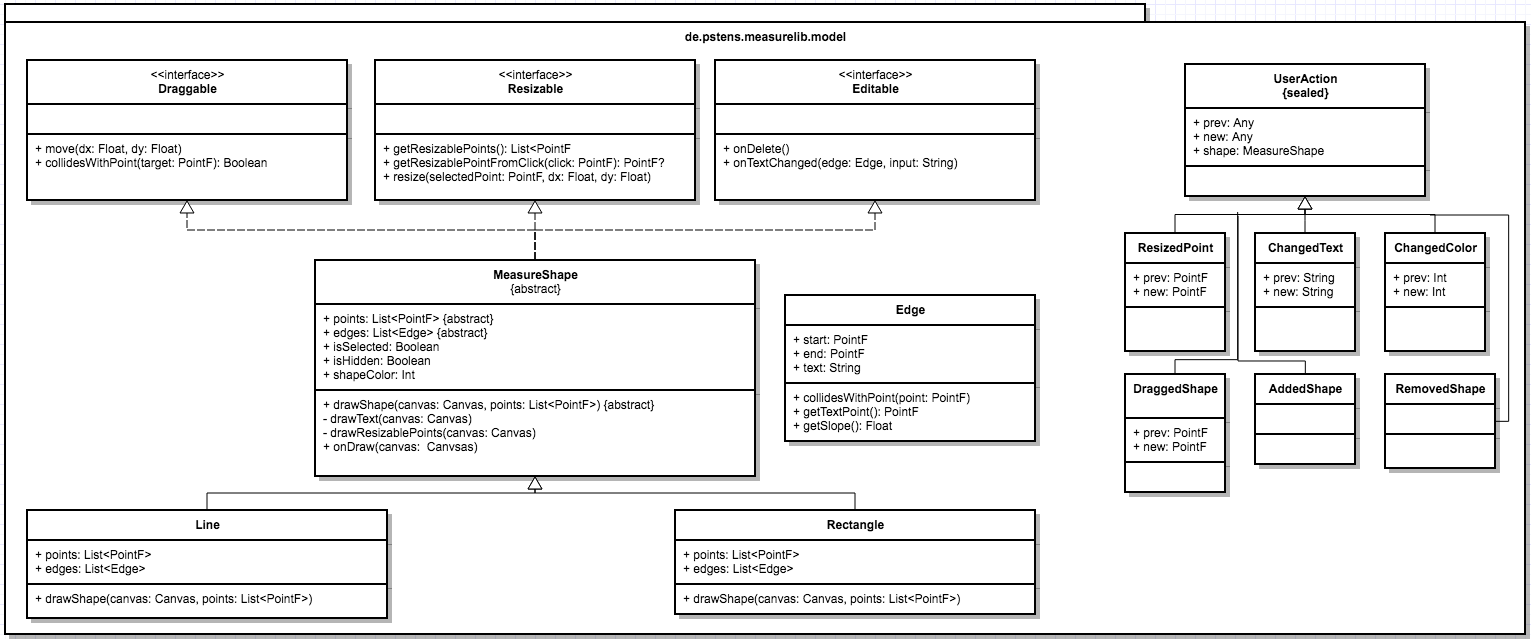
\includegraphics[keepaspectratio, width=\textwidth]{prototype1/model}
  \caption{Datenmodell (Model)}
  \label{fig:model}
\end{figure}

\begin{figure}[h]
  \centering
  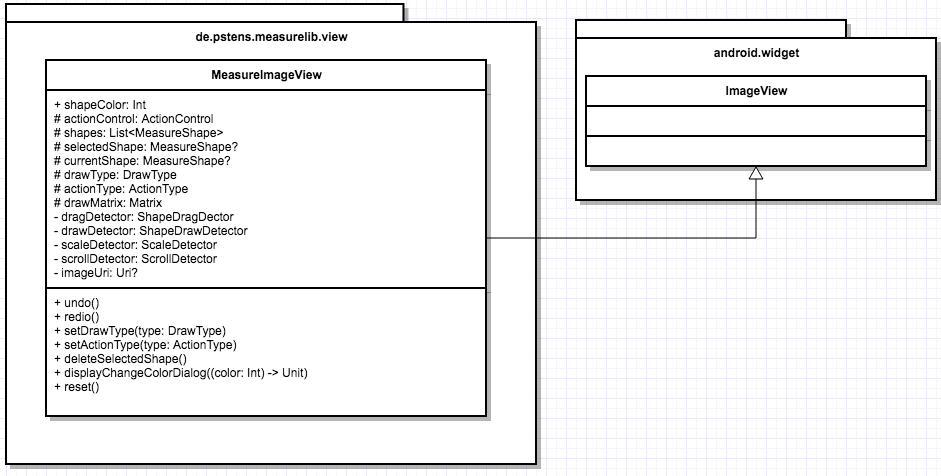
\includegraphics[keepaspectratio, width=\textwidth]{prototype1/view}
  \caption{Präsentationskomponente (View)}
  \label{fig:view}
\end{figure}

\begin{figure}[h]
  \centering
  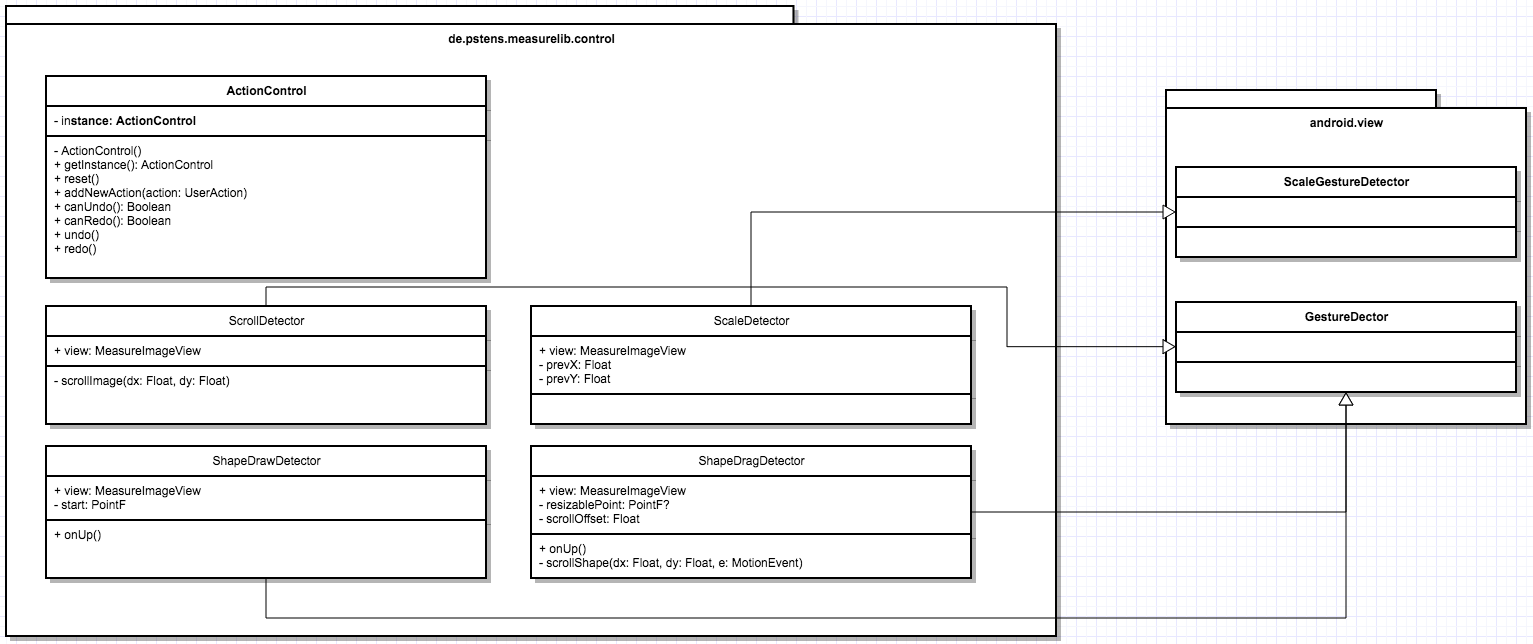
\includegraphics[keepaspectratio, width=\textwidth]{prototype1/control}
  \caption{Programmsteuerung (Control)}
  \label{fig:control}
\end{figure}

\chapter{Verbreitung der verschiedenen Android-Versionen Dezember 2017}
\begin{figure}[h]
  \centering
  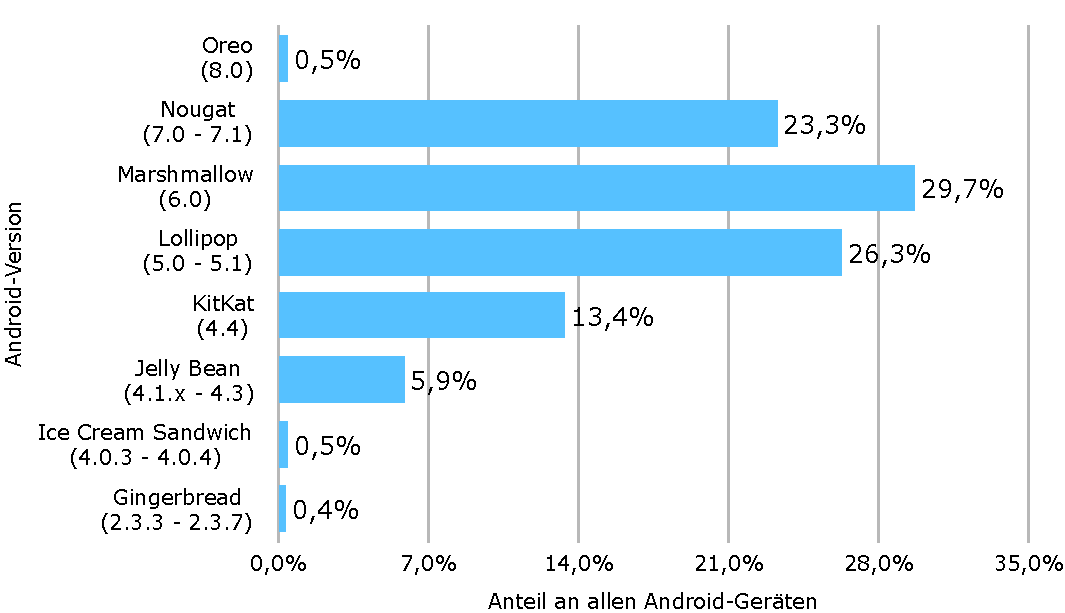
\includegraphics[keepaspectratio, width=\textwidth]{prototype2/androidchart}
  \caption{Anteil der verschiedenen Android-Versionen an allen Geräten mit Android OS weltweit im Zeitraum vom 5. bis 11. Dezember 2017}
  \label{fig:versionchart}
\end{figure}
